\label{capitolo1}
\section*{Introduzione}
Il corso di Architetture Avanzate dei Calcolatori si prefigge lo scopo di fornire una vista sulle più recenti architetture avanzate dei calcolatori, introducendo i meccanismi base delle micro-architetture che si possono ritrovare nei moderni microprocessori, ed infine fornire le ragioni dietro alle tecniche adottate nelle architetture dei computer.
\section{Pipelining}
\subsection{Concetti base}
Definiamo prima di tutto quali sono le principali caratteristiche dell'architettura MIPS partendo dalla definizione delle istruzioni utilizzate dai calcolatori.
Esistono due tipi di istruzioni le MISC e le RISC; le istruzioni \textbf{RISC} (\emph{Reduced Instruction Set Computer}) sono istruzioni semplici che posssono essere eseguite in un unico ciclo di clock e ottimizzate per le performance sulle CPU CISC.
Le architetture MISC sono solitamente di tipo \emph{LOAD/STORE}, ovvero gli operandi della ALU arrivano da dei registri posti nella CPU e non direttamente caricati dalla memoria,  questa caratteristica richiede che siano necessarie due particolari istruzioni:
\begin{itemize}
\item \textbf{load} che carica i dati dalla memoria ai registri
\item \textbf{store} che sposta i dati dai registri alla memoria
\end{itemize}
Infine altra caratteristica fondamentale per le architetture MISC è l'utilizzo della \emph{Pipeline} una tecnica di ottimmizzazione basata sull'esecuzione sovrapposta di molteplici istruzioni sequenziali.
\subsubsection{Reduced Instruction Set nei processori MIPS}
Vediamo ora quali sono le diverse istruzzioni di tipo RISC e come sono rappresentate nel calcolatore
\paragraph{Istruzioni ALU}
Vediamo innanzitutto le istruzioni di somma ovvero quelle eseguite dalla ALU. Possono essere di due tipi, una somma tra due registri oppure una somma con un indice prestabilito (utile ad esempio per spostarsi con gli array o nei cicli).
Vediamo lo pseudo codice assembly
\begin{verbatim}
add  $s1, $s2, $s3      # $s1 <- $s2 + $s3
addi $s1, $s2, 4        # $s1 <- $s2 + 4
\end{verbatim}
Mentre in \figurename~\ref{fig:regALU} vediamo come è suddivisa un'istruzione in un registro nel caso di somma tra due registri.
\begin{figure}[htb]
\centering
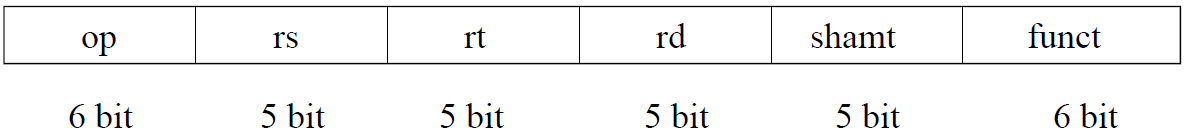
\includegraphics[scale=0.5]{img/regALU.png}
\caption{Divisione delle informazioni in un registro di un istruzione ALU di tipo registro-registro}\label{fig:regALU}
\end{figure}
I diversi campi indicano rispettivamente:
\begin{description}
\item[op] identifica il tipo di istruzione ALU da eseguire
\item[rs] indica il registro nel quale è contenuto il primo operando
\item[rt] indica il registro nel quale è contenuto il secondo operando
\item[rd] indica il registro di destinazione
\item[shamt] sta ad indicare i bit di shift amount
\item[funct] identifica i diversi tipi di istruzione
\end{description}
\begin{figure}[htb]
\centering
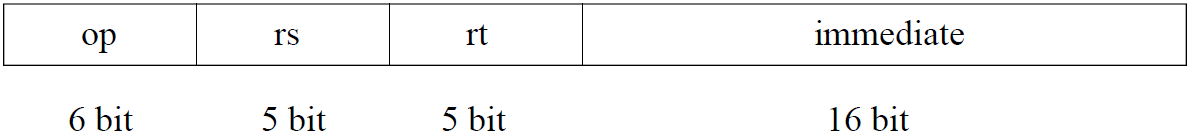
\includegraphics[scale=0.5]{img/ALUdir.png}
\caption{Divisione delle informazioni in un registro di un istruzione ALU di tipo diretto}\label{fig:ALUdir}
\end{figure}
Nella \figurename~\ref{fig:ALUdir} vediamo invece la suddivisione di un registro nel caso di un operazione di ALU immediata.
La suddivisione dei diversi campi è la seguente:
\begin{description}
\item[op] identifica l'istruzione di tipo immediato
\item[rs] indica il registro nel quale è posizionato il primo operando
\item[rt] indica il registro di destinazione del risultato
\item[immediate] contiene il valore per l'operazione immediata nel range $-2^{15}$ e $+2^{15}-1$
\end{description}
\paragraph{Istruzioni LOAD/STORE}
Le istruzioni di \emph{load} e di \emph{store} sono quelle che permettono di caricare e scaricare i valori dai registri della CPU alla memoria centrale e viceversa.
Una suddivisione dei registri per quanto riguarda le istruzioni di load e store è identificata in \figurename~\ref{fig:loadstore}.\\
\begin{figure}[htb]
\centering
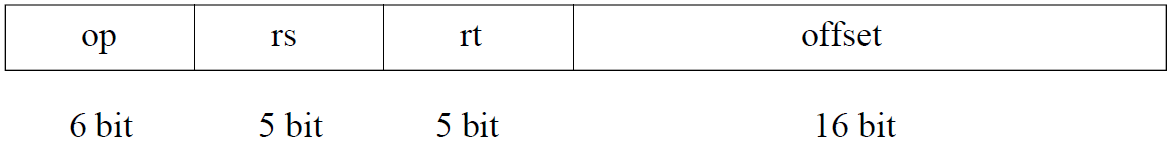
\includegraphics[scale=0.5]{img/loadstore.png}
\caption{Divisione delle informazioni in un registro di un istruzione tipo load/store}\label{fig:loadstore}
\end{figure}
La suddivisione del registro è la seguente:
\begin{description}
\item[op] identifica l'istruzione di tipo load o store
\item[rs] identifica il registro base
\item[rt] identifica il registro sorgente o destinazione per i dati delle operazioni di store o di load da o per la memoria
\item[offset] da sommare all'indirizzo contenuto in \emph{rs} per calcolare l'indirizzo di memoria
\end{description}
\paragraph{Istruzioni di salto}
Le istruzioni di salto sono di due tipi, possiamo avere istruzioni di salto condizionato oppure istruzioni di salto incondizionato.
Per quanto riguarda il salto condizionato si ha quando si decide se saltare ad una determinata istruzione in base al valore di una condizione. Lo pseudo assembly di tale istruzione è:
\begin{verbatim}
beq $s1, $s2, L1
\end{verbatim}
che corrisponde alla condizione "se \$s1 = \$s2 allora salta all'etichetta L1".
La suddivisione del registro per questo tipo  di istruzione è mostrata in \figurename~\ref{fig:condbranch}\\
\begin{figure}[htb]
\centering
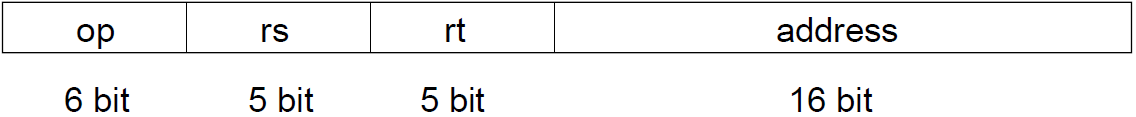
\includegraphics[scale=0.5]{img/condbranch.png}
\caption{Divisione delle informazioni in un registro di un istruzione tipo branch condizionato}\label{fig:condbranch}
\end{figure}
\begin{description}
\item[op] identifica l'istruzione di tipo branch condizionale
\item[rs] identifica il primo registro da comparare
\item[rd] identifica il secondo registro da comparare
\item[address] identifica l'offsett rispetto al PC che corrisponde all'indirizzo dell'etichetta
\end{description}
Per quanto riguarda il salto incondizionato il funzionamento è molto più semplice, quando si raggiunge l'istruzione di salto il PC punta direttamente all'istruzione indicata dall'etichetta.\\
Un esempio di suddivisione dei registri è rappresentato in \figurename~\ref{fig:uncondbranch} 
\begin{figure}[htb]
\centering
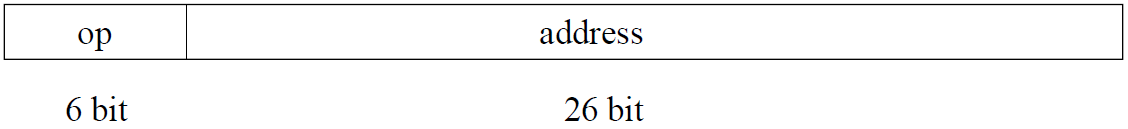
\includegraphics[scale=0.5]{img/uncondbranch.png}
\caption{Divisione delle informazioni in un registro di un istruzione tipo branch incondizionato}\label{fig:uncondbranch}
\end{figure}
dove i valori indicano rispettivamente
\begin{description}
\item[op] identifica il tipo di istruzione
\item[address] identifica l'indirizzo della prossima istruzione da eseguire
\end{description}
Possiamo suddividere le operazioni in tre categorie in base a come vengono eseguite:
\begin{itemize}
\item Tipo R (\emph{Registro})
\begin{itemize}
\item Istruzione ALU
\end{itemize}
\item Tipo I (\emph{Immediate})
\begin{itemize}
\item ALU immediate
\item Istruzioni Load/Store
\item Istruzioni di salto condizionato
\end{itemize}
\item Tipo J (\emph{jump})
\begin{itemize}
\item Istruzioni di salto incondizionato
\end{itemize}
\end{itemize}
Il perché di questa divisione lo si capisce molto facilmente dallo schema in \figurename~\ref{fig:rij} nel quale vengono confrontati le diverse suddivisioni degli Instruction Register.
\begin{figure}[htb]
\centering
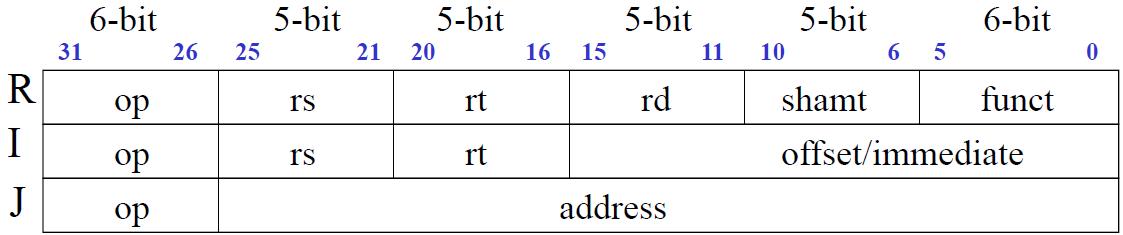
\includegraphics[scale=0.5]{img/rij.png}
\caption{Divisione dei registri nei diversi casi di operazione}\label{fig:rij}
\end{figure}
\subsubsection{Esecuzione delle istruzioni}
Vediamo ora come possono essere implementate le diverse istruzione in ambiente MIPS. Tutte le istruzioni possono essere implementati con almeno 5 cicli di clock nei quali vengono svolte le seguenti operazioni
\begin{enumerate}
\item \textbf{Instruction Fetch Cycle:} durante questo ciclo viene inviato il contenuto del \emph{Program Counter} all'\emph{Instruction Set} e aggiornare il PC alla prossima istruzione aggiungendo 4 al valore attuale (le istruzioni sono di 4 bytes)
\item \textbf{Instruction Decode and Register Read Cycle:} in questo ciclo si decodifica l'istruzione corrente e si leggono dal \emph{Register File} i registri necessari corrispondenti ai registri specificati nei campi dell'istruzione. Si fa inoltre l'estensione del segno nel caso sia necessario.
\item \textbf{Execution Cycle} In questo ciclo la ALU effettua le operazioni sugli elementi che sono stati preparati nel ciclo precedente. In base alle istruzioni la ALU esegue le seguenti operazioni
\begin{itemize}
\item Istruzione ALU registro-registro: la ALU esegue le operazioni sugli operandi che ha letto dal \emph{Register File}
\item Istruzioni ALU immediate: la ALU esegue l'operazione specificate sul primo operando letto dal \emph{Register File} e sul operando immediato al quale è stata applicata l'estensione di segno.
\item Istruzioni Load/Store la ALU aggiunge all'indirizzo base l'offset per calcolare l'indirizzo effettivo.
\item Istruzioni di salto condizionato: la ALU compara i due registri e calcola l'indirizzo target del salto e incrementa il PC
\end{itemize}
\item \textbf{Memory Access (ME):} durante questo ciclo le istruzioni di \emph{Load} effettuano la lettura dalla memoria usando l'indirizzo effettivo calcolato al ciclo precedente, le istruzione di \emph{Store} scrivono nella memoria i dati provenienti dal registro, infine, le istruzioni di \emph{Branch}  aggiornano il valore del Program Counter con l'indirizzo target
\item \textbf{Write-Back Cycle (WB):} in questo ciclo le istruzioni di \emph{Load} scrivono i dati letti dalla memoria nel registro di destinazione mentre le istruzioni di \emph{ALU} scrivono il risultato delle operazioni nei registri di destinazione.
\end{enumerate}
Come possiamo notare le diverse operazioni non usano sempre tutti i cicli appena descritti ma solitamente (tranne nel caso della \emph{load}) attraversano solo alcune fasi come possiamo vedere dallo schema in \figurename~\ref{fig:cicli}.\\
Mentre nella tabella di \figurename~\ref{fig:latency} possiamo vedere le latenze di ogni operazione nel caso di tempo di ciclo uguale ad 1 secondo.
\begin{figure}[htb]
\centering
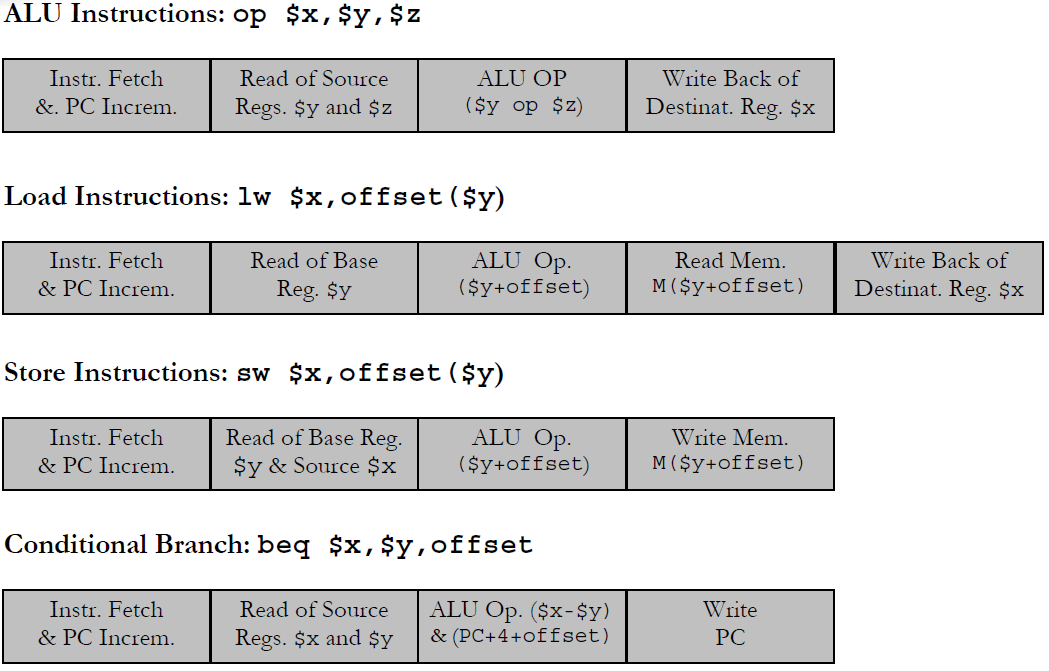
\includegraphics[scale=0.5]{img/cicli.png}
\caption{Cicli eseguiti da ogni operazione}\label{fig:cicli}
\end{figure}
\begin{figure}[htb]
\centering
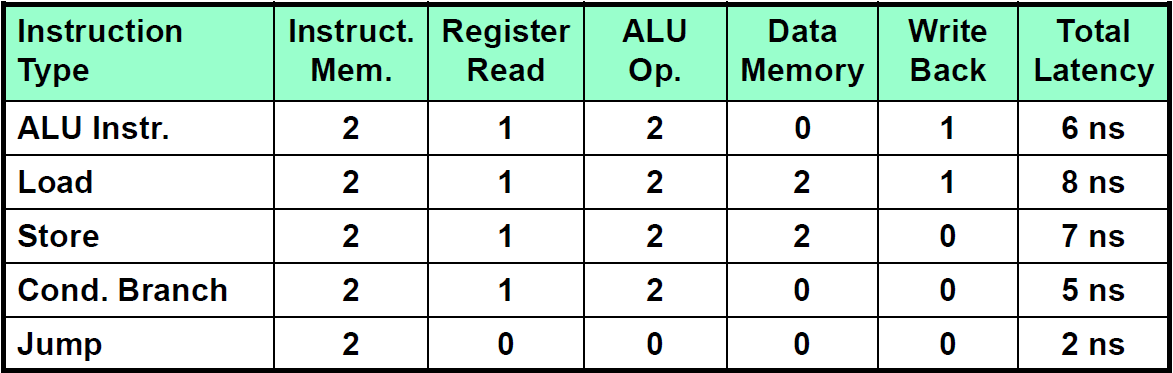
\includegraphics[scale=0.4]{img/latency.png}
\caption{Latenza delle diverse operazioni}\label{fig:latency}
\end{figure}
\subsubsection{Implementazione base di un MIPS}
Vediamo ora come potrebbe essere una semplice implementazione di un MIPS. Come notiamo dalla \figurename~\ref{fig:mips} abbiamo che la parte di memoria dedicata alle istruzioni (\emph{Instruction Memory}) è di sola lettura ed è separata dalla memoria dedicata ai dati (\emph{Data Memory}). Inoltre abbiamo 32 registri organizzati in un \emph{Register File} (RF) con 2 porte di lettura e una porta in scrittura.
\begin{figure}[htb]
\centering
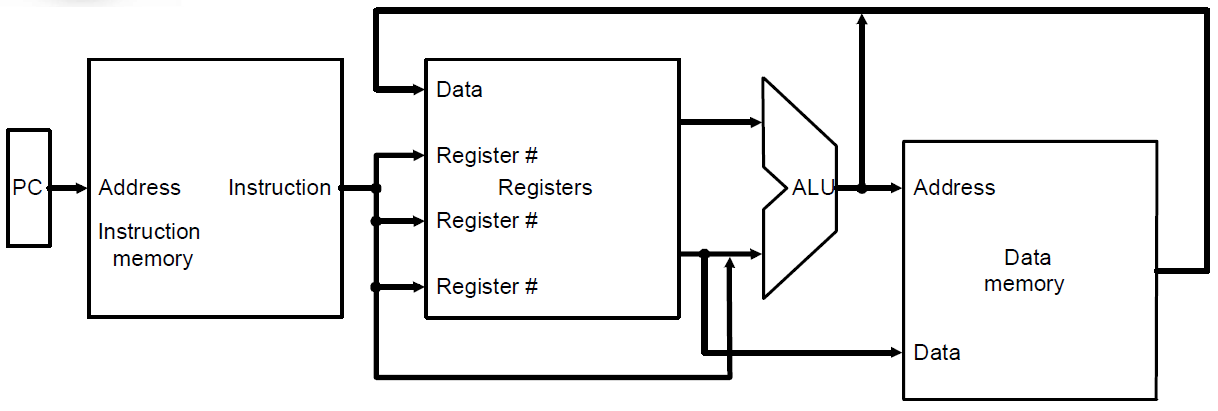
\includegraphics[scale=0.48]{img/mips.png}
\caption{Esempio di implementazione di MIPS}\label{fig:mips}
\end{figure}
Stabiliamo ora come viene implementato il clock del circuito; possiamo avere due possibilità, la prima è avere un unico ciclo di clock lungo quanto il percorso critico necessario per eseguire l'istruzione di load (la più lunga), la seconda è avere un ciclo di clock lungo quanto un singolo passaggio in uno dei componenti prima analizzati.\\
Analizziamo innanzitutto il caso di singolo ciclo, in questo caso il ciclo dovrà avere una durata pari al tempo necessario per eseguire un'istruzione di load che come abbiamo visto è pari a $T = 8 ns \quad (f=125 \ MHz)$. Assumiamo quindi che ogni istruzione verrà eseguita in un singolo ciclo di clock, ogni modulo verrà utilizzato una sola volta per clock e quei moduli che dovrebbero essere utilizzati più di una volta dovranno essere duplicati.
Inoltre dobbiamo tener conto anche delle differenze tra i diversi tipi di istruzioni, infatti, all'ingresso di scrittura dell'RF possiamo avere dati provenienti da una ALU e quindi di lunghezza [15-11] bit oppure dati provenienti da una load/store con una lunghezza di [20-16] bit questo richiede un \emph{Multiplexer} all'ingresso dei registri nel RF. In secondo luogo al secondo ingresso della ALU possiamo avere avere il dato proveniente da un registro nel caso di operazioni ALU oppure l'offset per le istruzioni di load/store, questo richiede un \emph{MUX} al secondo ingresso della ALU. Infine i dati all'output del Destination Register possono arrivare sia dal risultato della ALU oppure dal Data Memory nel caso di load questo comporta l'utilizzo di un \emph{MUX} all'ingresso in scrittura dei dati su RF.
In \figurename~\ref{fig:monocic} vediamo l'implementazione completa di un MIPS a ciclo singolo con l'introduzione, oltre che dei MUX precedentemente specificati, abche di due ALU (parte alta della figura) che permettono l'implementazione dei branch, e della logica di controllo (in rosso nella figura)\\
Veniamo ora al caso in cui il ciclo di clock sia di lunghezza pari al tempo necessario per un singolo modulo $T = 2 ns$ questo comporta che per eseguire un'istruzione di load sono necessari 5 cicli di clock. Ogni fase dell'istruzione richiede un ciclo di clock ma questo permette la condivisione dei moduli tra diverse istruzioni in differenti cicli di clock, anche se questo richiede l'inserimento di registri tra un unità  e l'altra.
\begin{figure}[!Hptb]
\centering
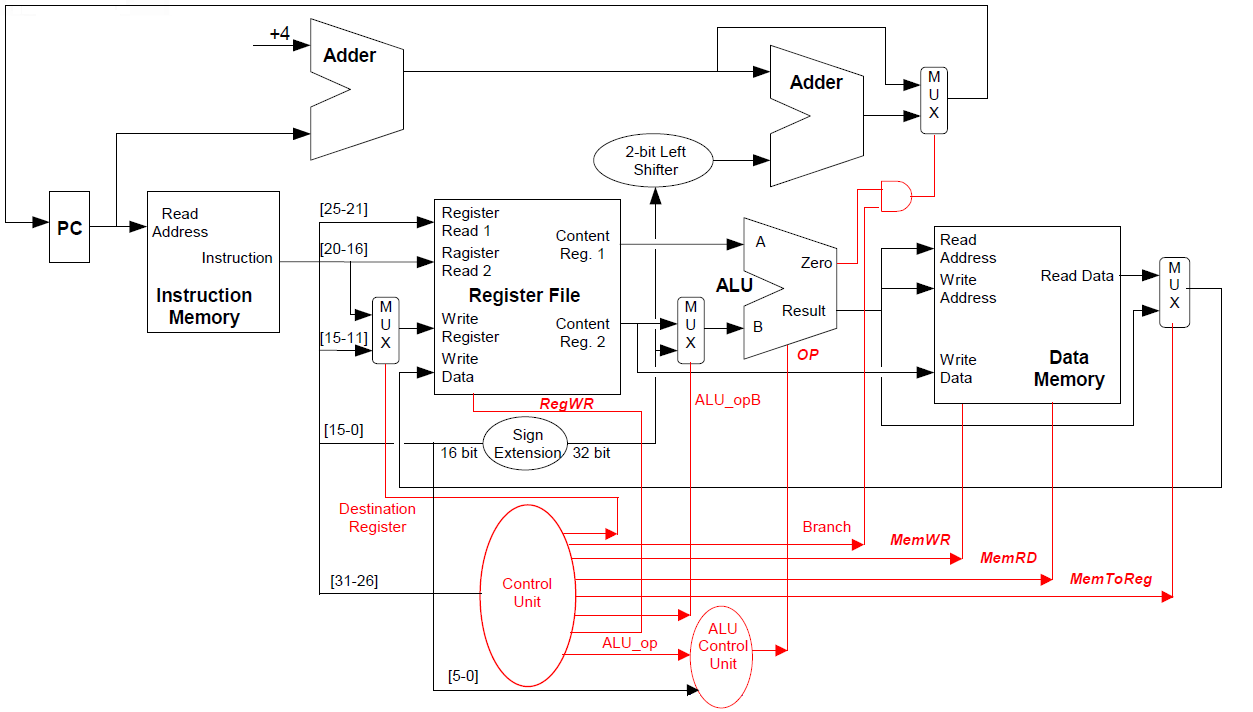
\includegraphics[scale=0.67, angle=90]{img/monocic.png}
\caption{MIPS a singolo ciclo con logica di controllo}\label{fig:monocic}
\end{figure}
\subsection{Pipelining}
Il pipelining è una tecnica di ottimizzazione basata sull'esecuzione multipla sovrapposta di istruzioni sequenziali. L'idea fondamentale è quella di sfruttare il parallelismo intriseco delle istruzioni sequenziali in quanto l'esecuzione di una istruzione è suddivisa in fasi differenti (\emph{pipelines stages}) che richiedono soltanto una piccola frazione di tempo per essere completate. I diversi stati sono connessi in sequenza nella pipeline, un'istruzione entra da una parte procede attraverso i diversi stadi e esce all'altro capo come in una catena di montaggio.\\
I vantaggi di questa tecnica è che è completamente trasparente al programmatore  inoltre come in una catena di montaggio il tempo necessario per eseguire un'istruzione è uguale al caso in cui l'istruzione sia eseguita senza pipeline. Quello che la pipeline fa non è ridurre il tempo di esecuzione ma incrementare il numero di istruzioni eseguite contemporaneamente e perciò aumentare la frequenza di completamento come vediamo in \figurename~\ref{fig:seqvspipe}\\
\begin{figure}[tb]
\centering
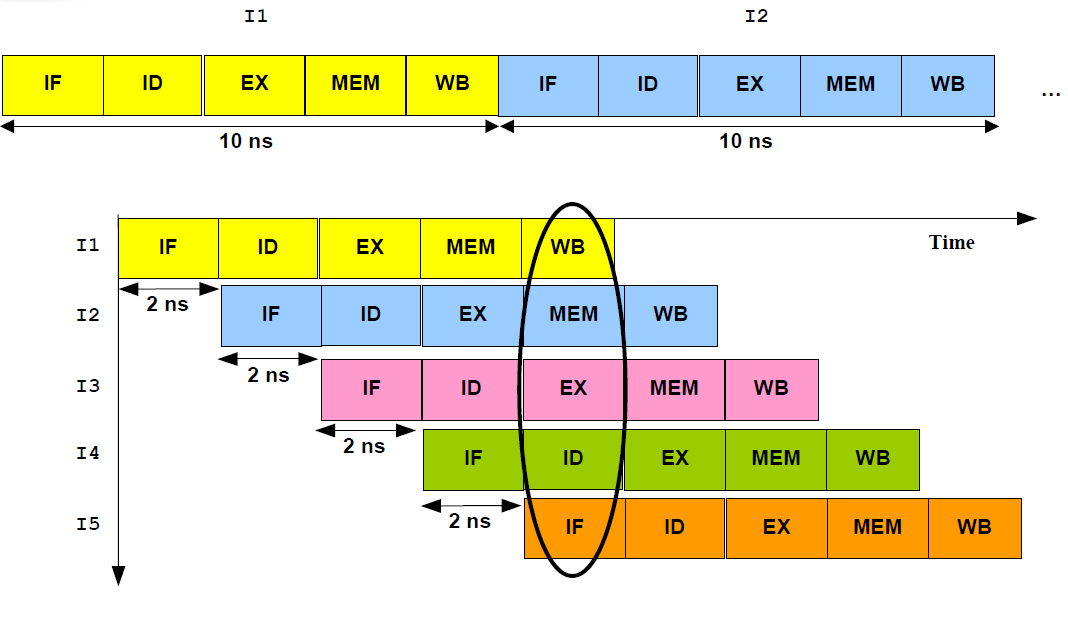
\includegraphics[scale=0.45]{img/seqvspipe.png}
\caption{Confronto tra esecuzione sequenziale e pipelined}\label{fig:seqvspipe}
\end{figure}
Il tempo necessario per far avanzare un'istruzione di una fase corrisponde ad un ciclo di clock, le diverse fasi perciò devono essere \emph{sincronizzate}, il periodo di clock deve essere uguale al tempo di esecuzione della fase più lenta (nel nostro esempio 2ns). L'obiettivo è quello di bilanciare la lunghezza di ogni fase della pipeline in modo da avere uno \emph{speedup ideale} uguale al numero di fasi della pipeline.\\
Nel caso ideale vediamo come la pipeline sia più efficiente sia dell'architettura a singolo ciclo che a quella multi-ciclo viste in precedenza.
Nel caso di una CPU1 non pipeline con un unico ciclo di clock della durata di 8ns contro una CPU2 con una pipeline a 5 stadi e ciclo di 2ns abbiamo che:
\begin{itemize}
\item la \emph{latenza} ovvero il tempo necessario per una istruzione è peggiore nel caso di CPU2: 8ns vs 10ns
\item il \emph{throughput} è notevolmente migliorato: $1 \ istruzione/8ns$ vs $1 \ istruzione/2ns$
\end{itemize}
Nel caso di CPU3 multi-ciclo senza pipeline contro un'architettura CPU2 descritta in precedenza abbiamo:
\begin{itemize}
\item la \emph{latenza} resta invariata: 10 ns
\item il \emph{throughput} cresce di ben 5 volte: $1 \ istruzione/10ns$ vs $1 \ istruzione/2ns$
\end{itemize}
\subsubsection{Implementazione di una Pipeline}
Innanzitutto vediamo quali fasi devono attraversare ciascuna operazione in quanto non tutte le fasi sono necessarie per tutte le operazioni, uno schema riassuntivo è specificato in \figurename~\ref{fig:pipefasi}. \\
\begin{figure}[tbh]
\centering
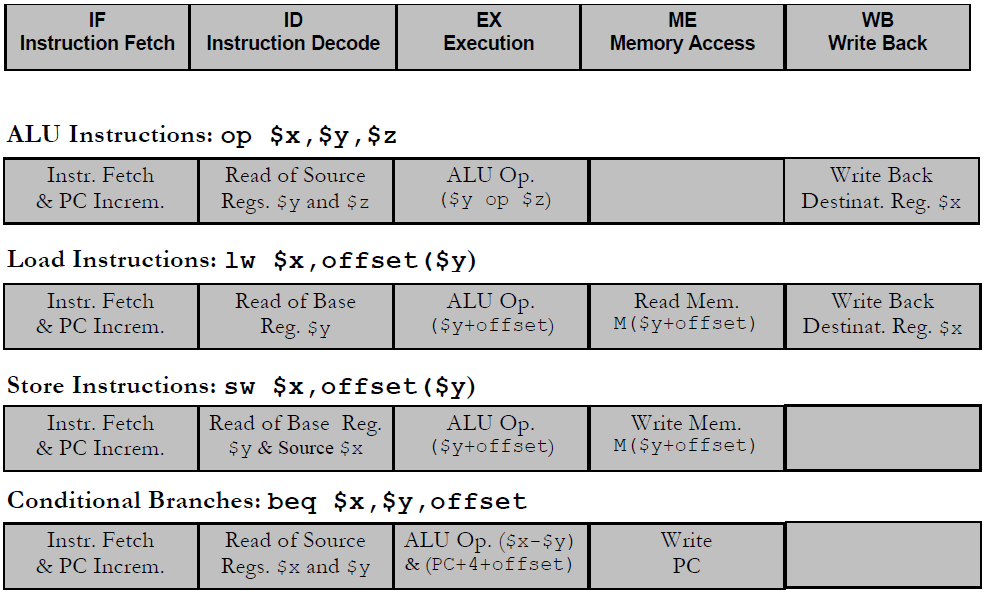
\includegraphics[scale=0.45]{img/pipefasi.png}
\caption{Fasi della pipeline necessarie ad ogni istruzione}\label{fig:pipefasi}
\end{figure}
La divisione dell'esecuzione di una istruzione in 5 fasi implica che in ogni ciclo di clock cinque istruzione sono in esecuzione questo comporta la necessità di inserire dei \emph{registri} tra una fase e l'altra della pipeline per separare i diversi stage.\\
In \figurename~\ref{fig:pipeline} vediamo una possibile implementazione di un'architettura MIPS pipelined con l'introduzione dei registri tra le fasi (in verde).
\begin{figure}[!Htb]
\centering
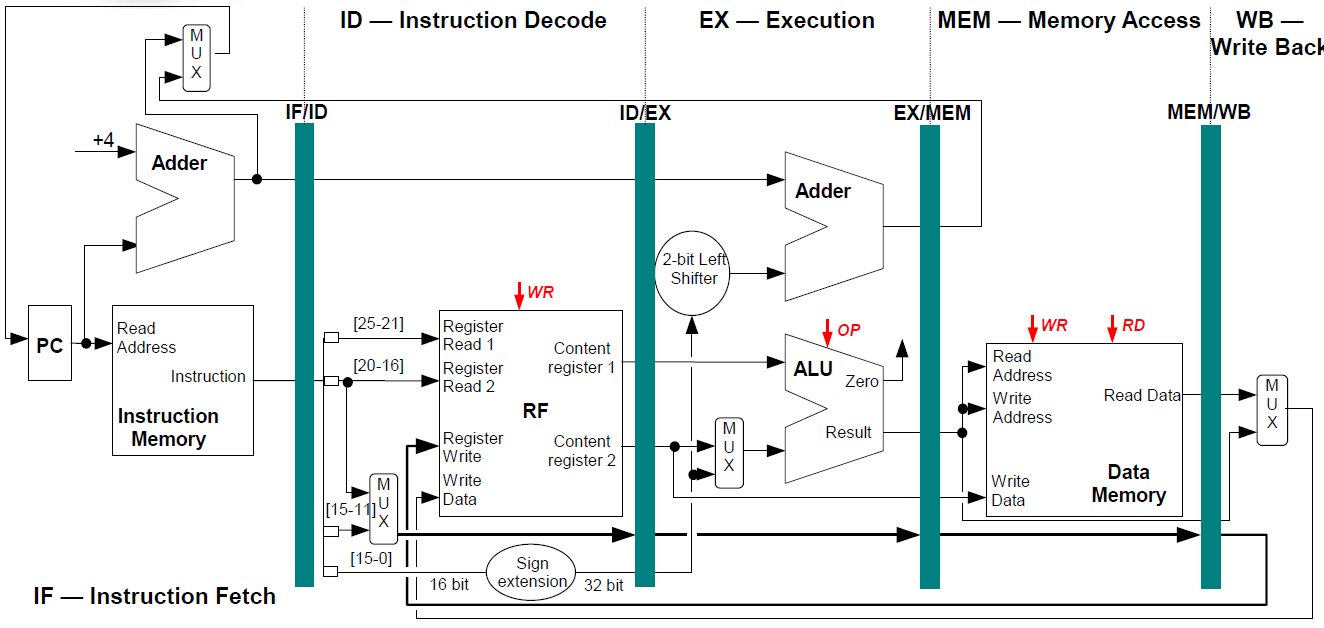
\includegraphics[scale=0.6, angle=90]{img/pipeline.png}
\caption{Schema di un MIPS con pipeline}\label{fig:pipeline}
\end{figure}
\subsection{Il problema del ''Hazard''}
Si ha un \emph{hazard} quando vi è una dipendenza tra istruzioni diverse e la sovrapposizione dovuta al pipeline cambia l'ordine delle dipendenze sugli operandi. Hazard previene l'esecuzione della prossima istruzione nel ciclo di clock designato ma così facendo riduce le performance allontanandole dallo speedup ideale.\\
Possiamo distinguere tre classi di \emph{hazard}:
\begin{itemize}
\item \textbf{Structural Hazards:} si ha quando diverse istruzioni cercano di utilizzare la stessa risorsa simultaneamente (stessa memoria per istruzioni e dati)
\item \textbf{Data Hazards:} si ha quando si cerca di utilizzare un risultato prima che questo sia pronto(istruzione dipendente dalla precedente che è nella pipeline)
\item \textbf{Control Hazards:} si ha quando si deve prendere una decisione sulla esecuzione della prossima istruzione prima della valutazione di una condizione (branch condizionali)
\end{itemize}
Tra questi tre tipi di hazard il pimo non può presentarsi nelle architetture MIPS in quanto lo spazio di memoria dedicato alle istruzioni e quello dedicato ai dati sono fisicamente separati.
\pagebreak
\subsubsection{Data Hazard}
Per quanto riguarda il data hazard si verifica quando sono in esecuzione nella pipeline due o più istruzioni \emph{dipendenti}.
\begin{verbatim}
sub    $2, $1, $3
and   $12, $2, $5   #1° operando dipende dalla sub
or    $13, $6, $2   #2° operando dipende dalla sub
$add  $14, $2, $2   #1° & 2° operando dipendono dalla sub
sw    $15, 100($2)  #Il registro base dipende dalla sub
\end{verbatim}
Come vediamo dall'esempio in \figurename~\ref{fig:datahazard} abbiamo che le istruzioni successive alla sub debbono aspettare che la prima istruzione arrivi nella fase di \emph{write-back} prima di poter utilizzare il dato come avviene per l'ultima istruzione evidenziata da una freccia verde.
\begin{figure}[tb]
\centering
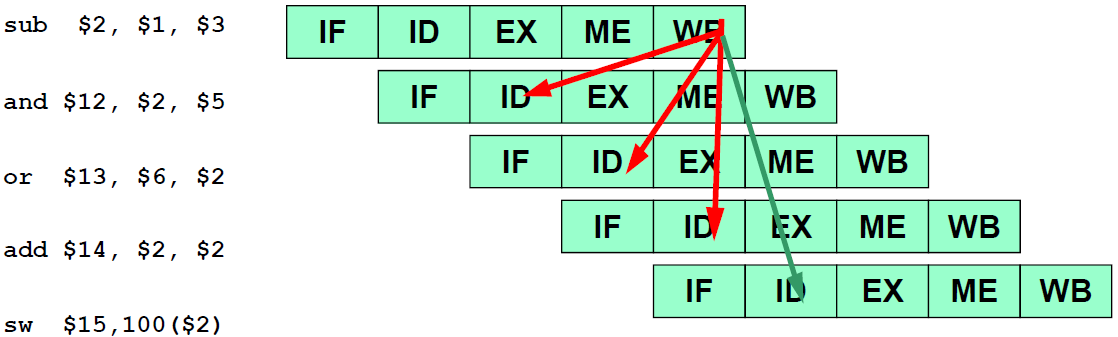
\includegraphics[scale=0.5]{img/datahazard.png}
\caption{Esempio di data hazard}\label{fig:datahazard}
\end{figure}
Esistono diversi meccanismi per far si che queste dipendenze vengano soddisfatte, le principali si possono suddividere in due categorie:
\begin{itemize}
\item \textbf{Tecniche di compilazione:} in questa categoria rientra il  re-scheduling dellle operazioni in modo da inserire istruzioni indipendenti tra le istruzioni correlate in modo da permettere il calcolo dei valori necessari; nel caso non sia possibile inserire altre operazioni il compilatore inserisce delle \texttt{nop} ovvero delle \emph{no operation}
\item \textbf{Tecniche hardware:} in questa categoria rientrano la possibilità di inserire delle \emph{bubbles} o degli stalli oppure le tecniche di \emph{Data Forwarding} e di \emph{Bypassing}
\end{itemize}
Vediamo innanzi tutto un esempio di inserimento di \texttt{nop} in \figurename~\ref{fig:nop}
\begin{figure}[tb]
\centering
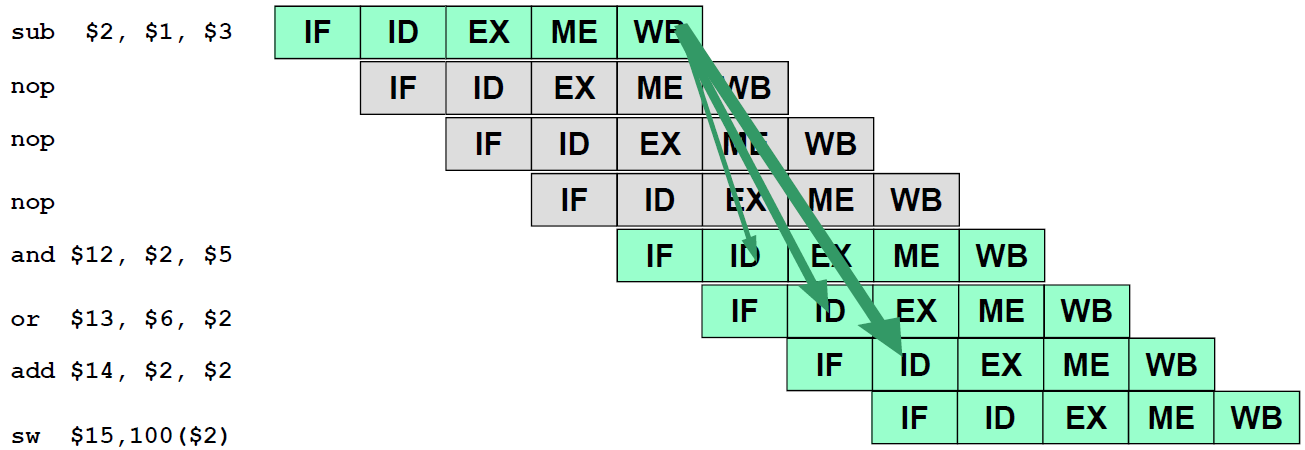
\includegraphics[scale=0.45]{img/nop.png}
\caption{Esempio di uso \texttt{nop}}\label{fig:nop}
\end{figure}
Come vediamo l'inserimento di nop perggiora lo speedup ideale.cosa che invece non succede se si applicano le tecniche di scheduling in quanto non vengono inserite istruzioni inutili nell'esecuzione  delle istruzioni ma viene modificato semplicemente l'ordine nel quale vengono eseguite.\\
Il caso di inserimento di stalli è molto simile a quello di inserimento delle nop la differenza sta nel fatto che si ferma l'esecuzione dell'istruzione dipendente il tempo necessario affinchè l'istruzione in esecuzione renda disponibile il dato come vediamo in \figurename~\ref{fig:stall}, ache in questo caso abbiamo un peggioramento dello speedup ideale.
\begin{figure}[tb]
\centering
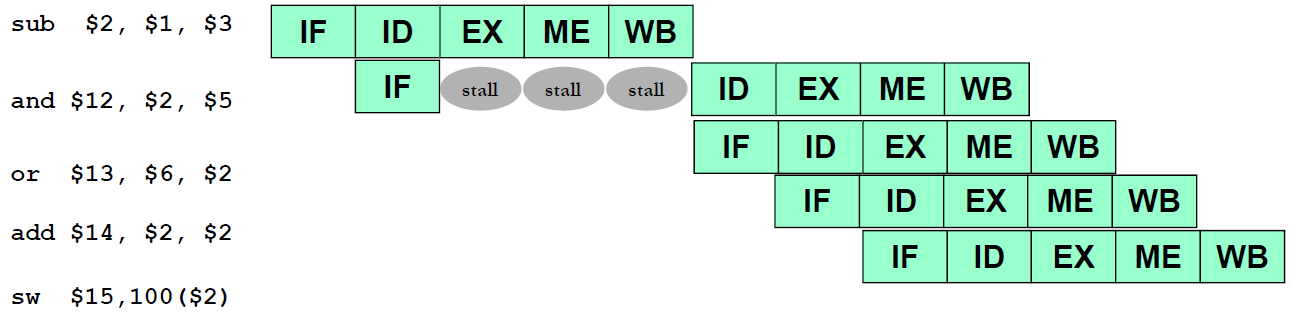
\includegraphics[scale=0.45]{img/stall.png}
\caption{Esempio di uso degli stalli}\label{fig:stall}
\end{figure}
\paragraph{Data Forwarding}
Il \emph{data forwarding} è una tecnica hardware che comporta l'utilizzo dei risultati temporanei immagazzinati nei registri della pipeline, per fare ciò abbiamo bisogno di aggiungere dei \emph{multiplexer} all'ingresso della ALU per selezionare gli ingressi. In \figurename~\ref{fig:forwardingpath} e \figurename~\ref{fig:forwardingcirc} vediamo uno schema riassuntivo dei collegamenti con i vari stadi dei multiplexere e lo schema hardware.
\begin{figure}[tb]
\centering
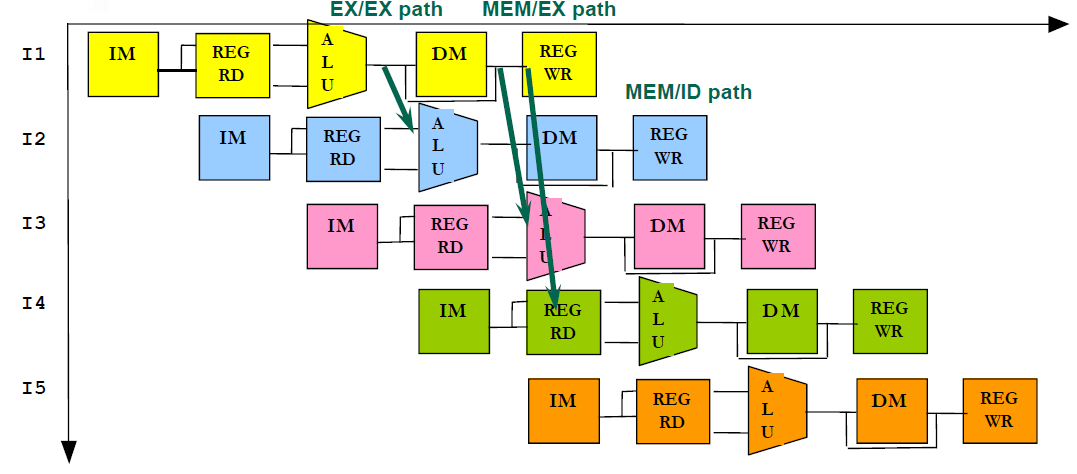
\includegraphics[scale=0.45]{img/forwardingpath.png}
\caption{Esempio di uso degli stalli}\label{fig:forwardingpath}
\end{figure}
Con l'architettura attuale nel caso di accesso sia in lettura che in scrittura su di uno stesso registro nello stesso ciclo di clock è necessario introdurre uno stallo nell'esecuzione. Nel caso, invece, di \emph{pipeline ottimizzata} possiamo assumere che la fase di lettura avviene nelle seconda metà del ciclo di clock mentre la fase di scrittura nella prima metà; in questo modo nel caso in cui lettura e scrittura facciano riferimento allo stesso registro non è necessario inserire stalli
\begin{figure}[!tb]
\centering
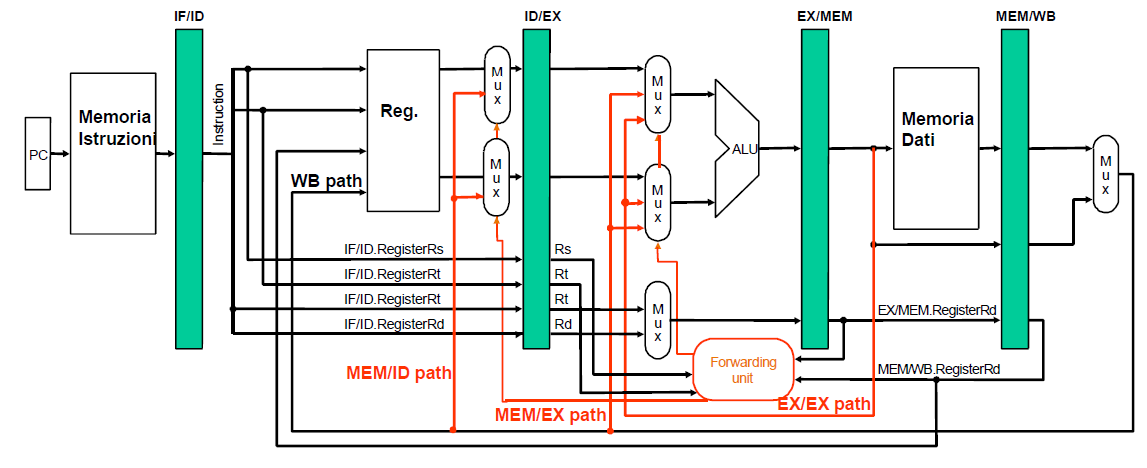
\includegraphics[scale=0.7,angle=90]{img/forwardingcirc.png}
\caption{Schema MIPS con forwarding}\label{fig:forwardingcirc}
\end{figure}
\pagebreak
\subsection{Analisi delle performance}
L'utilizzo della pipeline aumenta il throughput della CPU ma non riduce il tempo di esecuzione della singola istruzione, anzi solitamente aumenta la latenza di ogni istruzione bisogna quindi bilanciare il numero di fasi con l'overhead dovuto alla pipeline.\\
Definito $IC = Instruction \ Count$ possiamo determinare il numero di cicli di clock necessari per una operazione
$$\#Clock \ Cycle = IC + \# Stall \ Cycles + 4$$
$$CPI= Clock \ Per \ Instruction = \# Clock \ Cycle / IC = $$
$$(IC + \#Stall \ Cycles + 4)/IC$$
$$MIPS= f_{clock} / (CPI * 10^6)$$
Come visto fino ad ora la CPI ideale per la pipeline è 1 ma gli stalli degradano le performance.
Abbiamo così che la CPI media è data da:
$$Ave. \ CPI = Ideal \ CPI + \#Stall \ per \ Instruction$$
